\documentclass[xcolor=x11names,compress,professionalfonts]{beamer}

%% General packages %%%%%%%%%%%%%%%%%%%%%%%%%%%%%%%%%%
\usepackage[utf8]{inputenc}
\usepackage{psfrag}
\usepackage{graphicx}
\usepackage{tikz}
\tikzset{% change default arrow tips
    >=latex
}
\usepackage{ifthen}

\usepackage{amsmath}
\usepackage{nicefrac}

\usepackage{color}

%%%%%%%%%%%%%%%%%%%%%%%%%%%%%%%%%%%%%%%%%%%%%%%%%%%%%%


%% Beamer Layout %%%%%%%%%%%%%%%%%%%%%%%%%%%%%%%%%%
\useoutertheme[subsection=false,shadow]{miniframes}
\useinnertheme{rectangles}

\setbeamertemplate{navigation symbols}{}%remove navigation symbols

\newcommand{\btVFill}{\vskip0pt plus 1filll}%place an element at the bottom of the page

\usepackage{libertine}
\usepackage[T1]{fontenc}

\setbeamerfont{title like}{shape=\scshape}
\setbeamerfont{frametitle}{shape=\scshape}

\setbeamercolor*{lower separation line head}{bg=DeepSkyBlue4} 
\setbeamercolor*{normal text}{fg=black,bg=white} 
\setbeamercolor*{alerted text}{fg=red} 
\setbeamercolor*{example text}{fg=black} 
\setbeamercolor*{structure}{fg=black} 
 
\setbeamercolor*{palette tertiary}{fg=black,bg=black!10} 
\setbeamercolor*{palette quaternary}{fg=black,bg=black!10} 

\renewcommand{\(}{\begin{columns}}
\renewcommand{\)}{\end{columns}}
\newcommand{\<}[1]{\begin{column}{#1}}
\renewcommand{\>}{\end{column}}

\definecolor{BostonBlue}{HTML}{00688B}
\definecolor{Complementary}{HTML}{8B2300}

\renewcommand{\ss}[1]{\scriptsize{\text{#1}}}
%%%%%%%%%%%%%%%%%%%%%%%%%%%%%%%%%%%%%%%%%%%%%%%%%%

\usepackage{braket}
% compile child documents using this preamble
\usepackage{subfiles}

%%%My Math

\newcommand{\pd}[2]{\frac{\displaystyle \partial #1}{\displaystyle\partial #2}} % for partial derivatives
\renewcommand{\d}[1]{\mathrm{d}#1}

\begin{document}

\begin{frame}
\title{Fractal states on quasicrystals}

\author{ Nicolas Macé, Anuradha Jagannathan, \\ Frédéric Piéchon, Rémy Mosseri}

\institute % (optional)
{
  Laboratoire de Physique des Solides, Université Paris-Sud \\
  Laboratoire de Physique Théorique de la Matière Condensée, UPMC
}

\date{February 21, 2017}

\titlepage

\btVFill
\centering
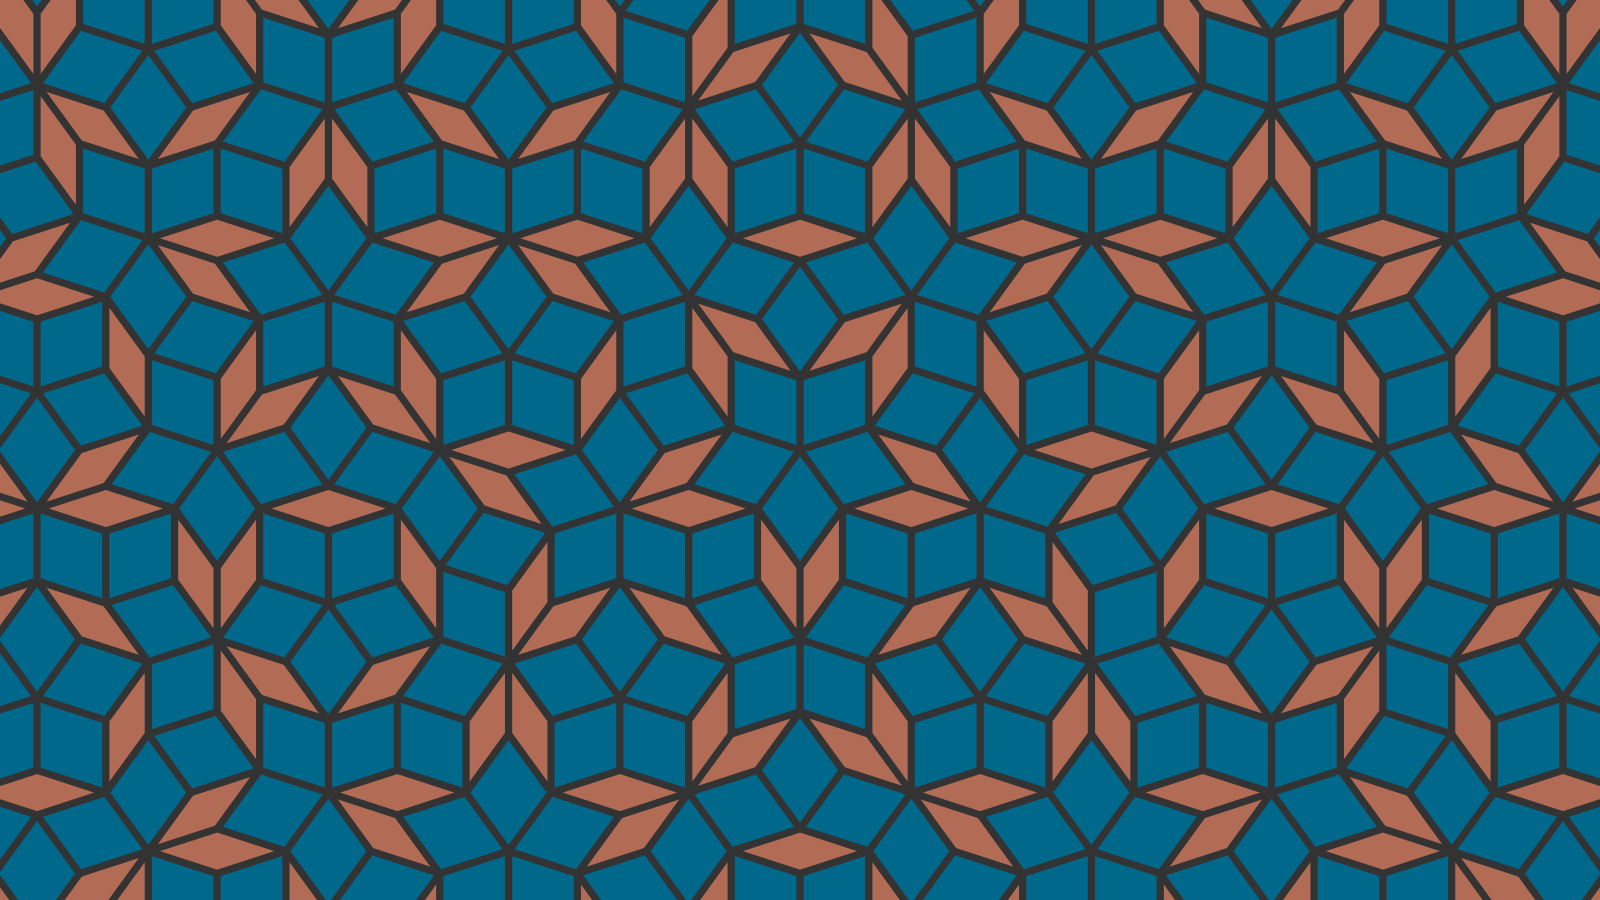
\includegraphics[scale=0.09]{img/cover.png}

\end{frame}

\begin{frame}
\frametitle{Outline}
\tableofcontents[hideallsubsections]
\end{frame}

\section{Quasicrystals and their physical properties}
%Each section needs a subsection for the small points on top to show up
\subsection{Dummy}
\begin{frame}{Les quasicristaux ?}
Un arrangement apériodique mais ``ordonné'' d'atomes/molécules/colloïdes

Plus précisément, un quasi a les propriétés suivantes :
\begin{itemize}
	\item il est \textbf{apériodique}
	\item il présente \textbf{un ordre à longue distance} (la diffraction révèle des pics nets)
\end{itemize}
\textbf{Les pavages quasipériodiques} modélisent les quasis.
\(
	\<{6cm}
		\centering
		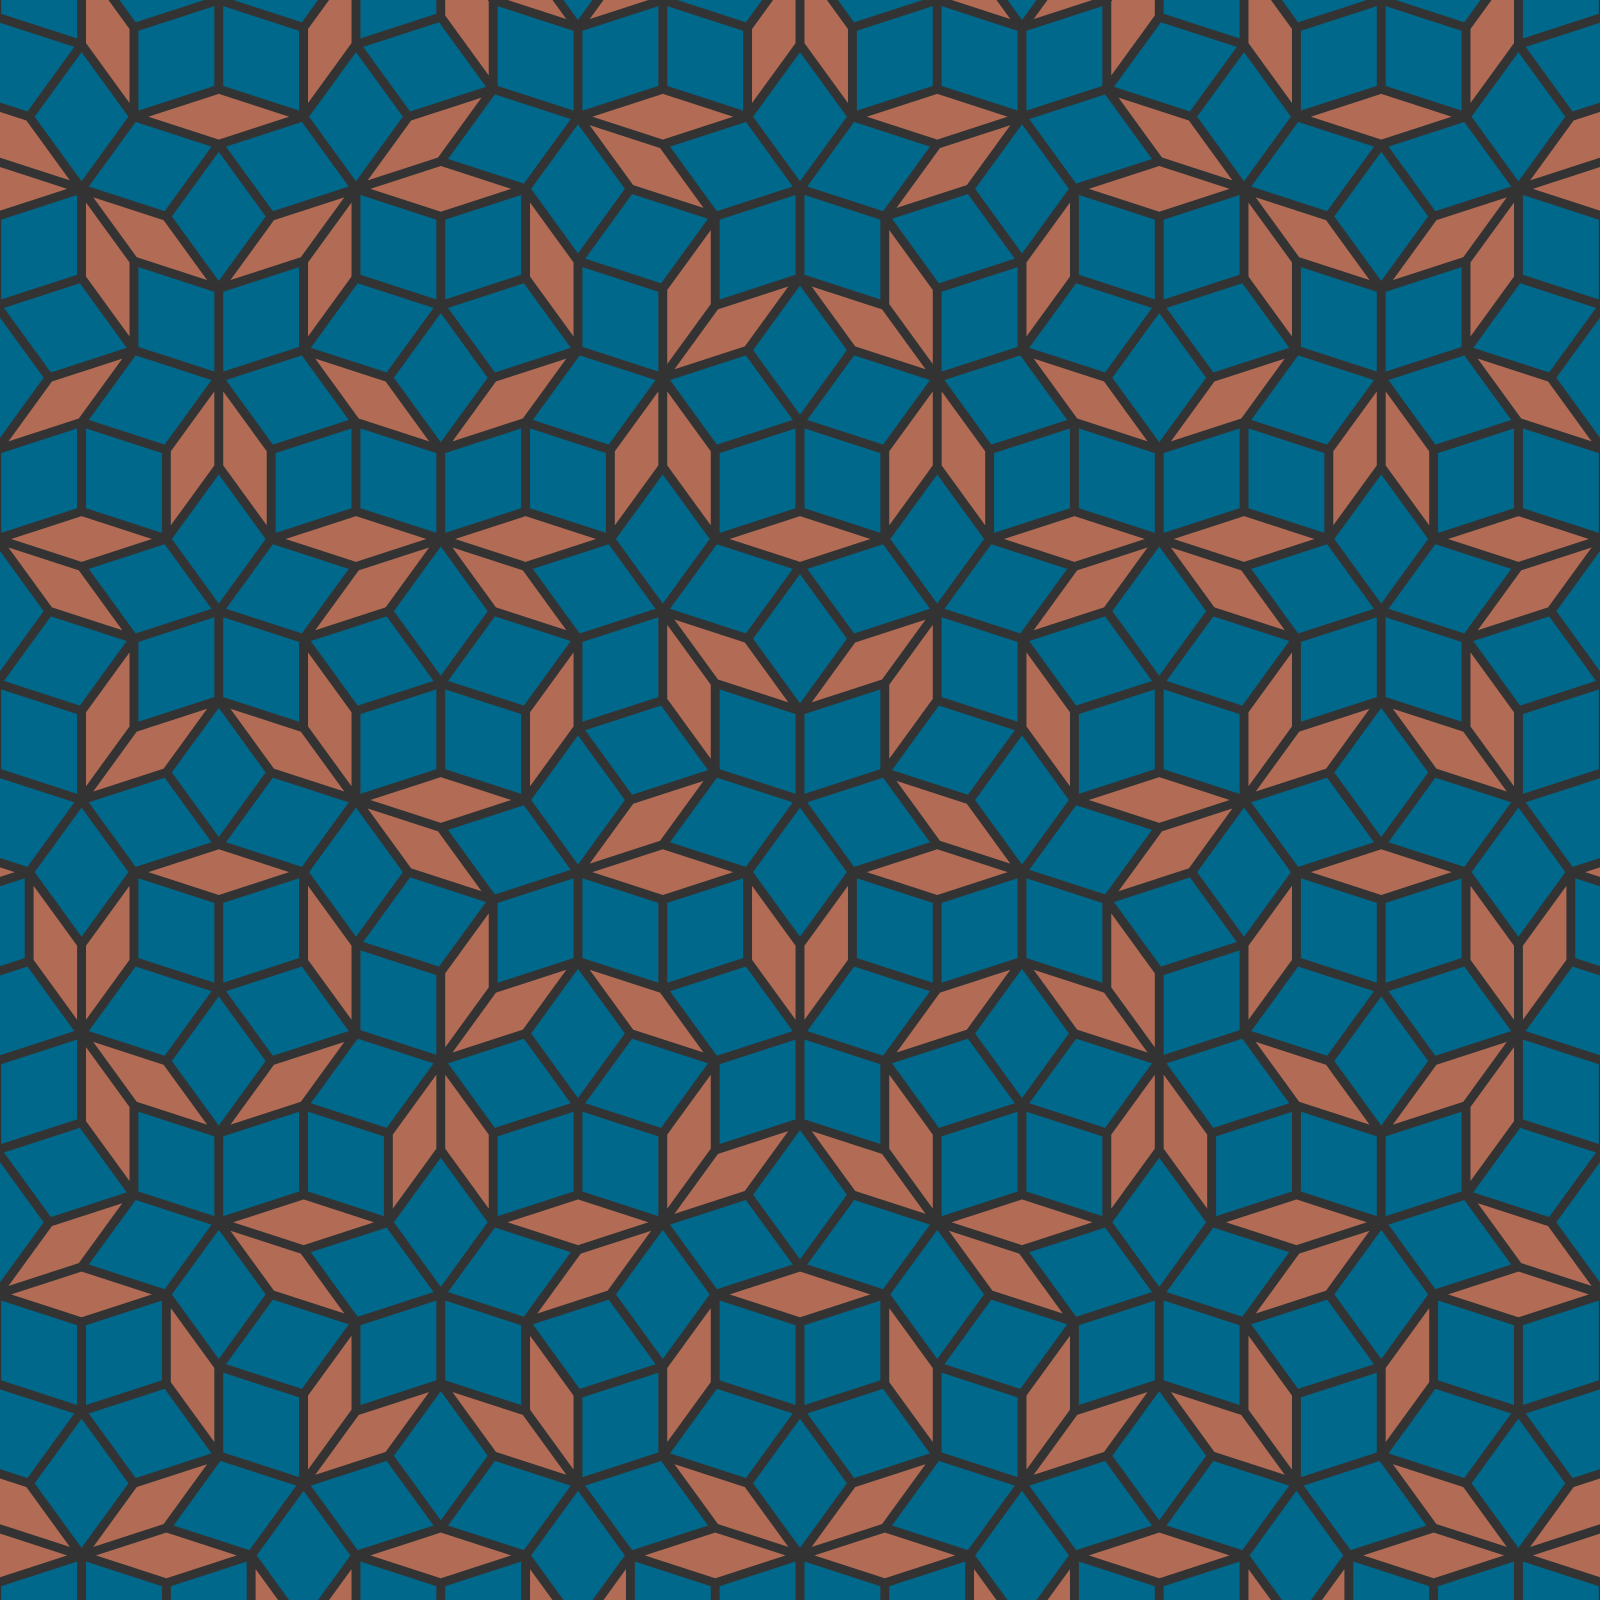
\includegraphics[scale=0.06]{img/penrose.png}
		
		\ss{Un morceau du pavage de Penrose,} \ss{souvent utilisé pour modéliser les quasis.}
	\>
	\<{6cm}
		\centering
		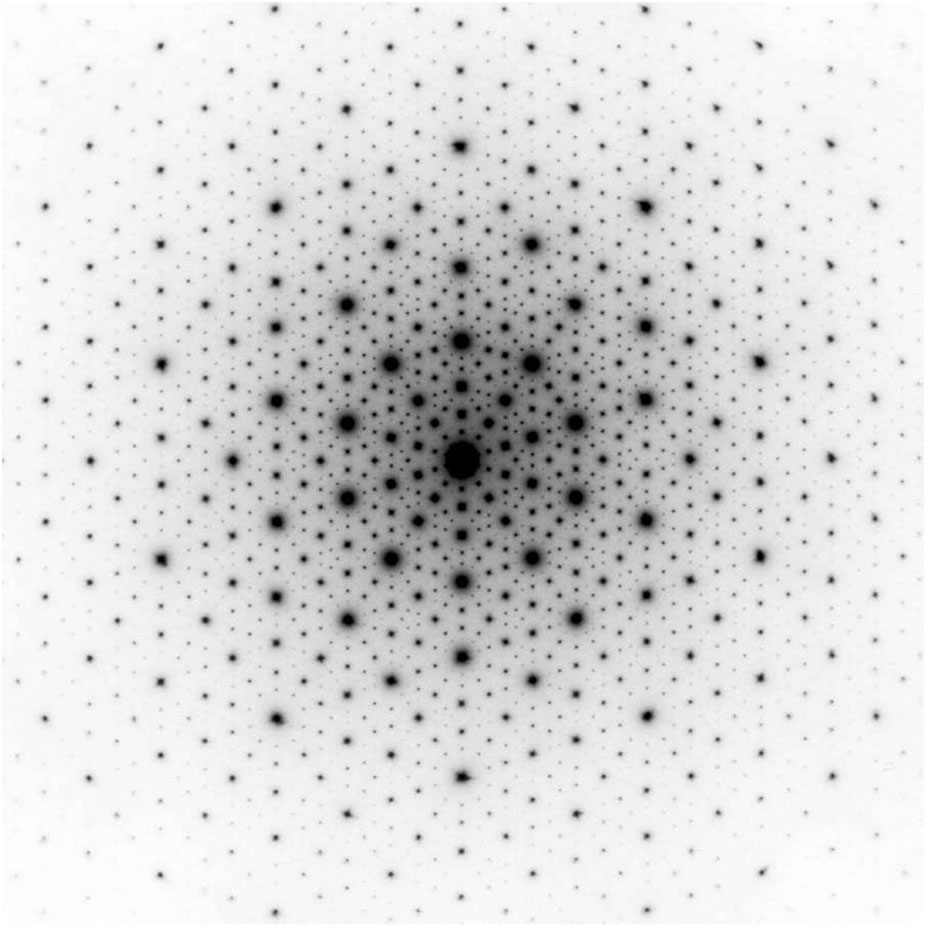
\includegraphics[scale=0.1]{img/diffraction_tenfold.png}
		
		\ss{Figure de diffraction d'un alliage d'AlPdMn} \ss{(groupe de Conradin Beeli)}
	\>
\)
\end{frame}

\begin{frame}{Exemples de quasicristaux}
\(
	\<{6cm}
		\centering
		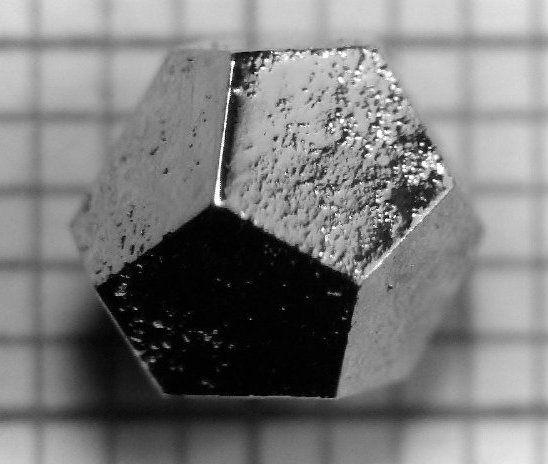
\includegraphics[scale=0.28]{img/homgzn.png}
		
		\ss{L'alliage HoMgZn alloy dans sa phase icosahédrale} \ss{(voir \url{doi:10.1038/nmat1244})}
	\>
	\<{6cm}
		\centering
		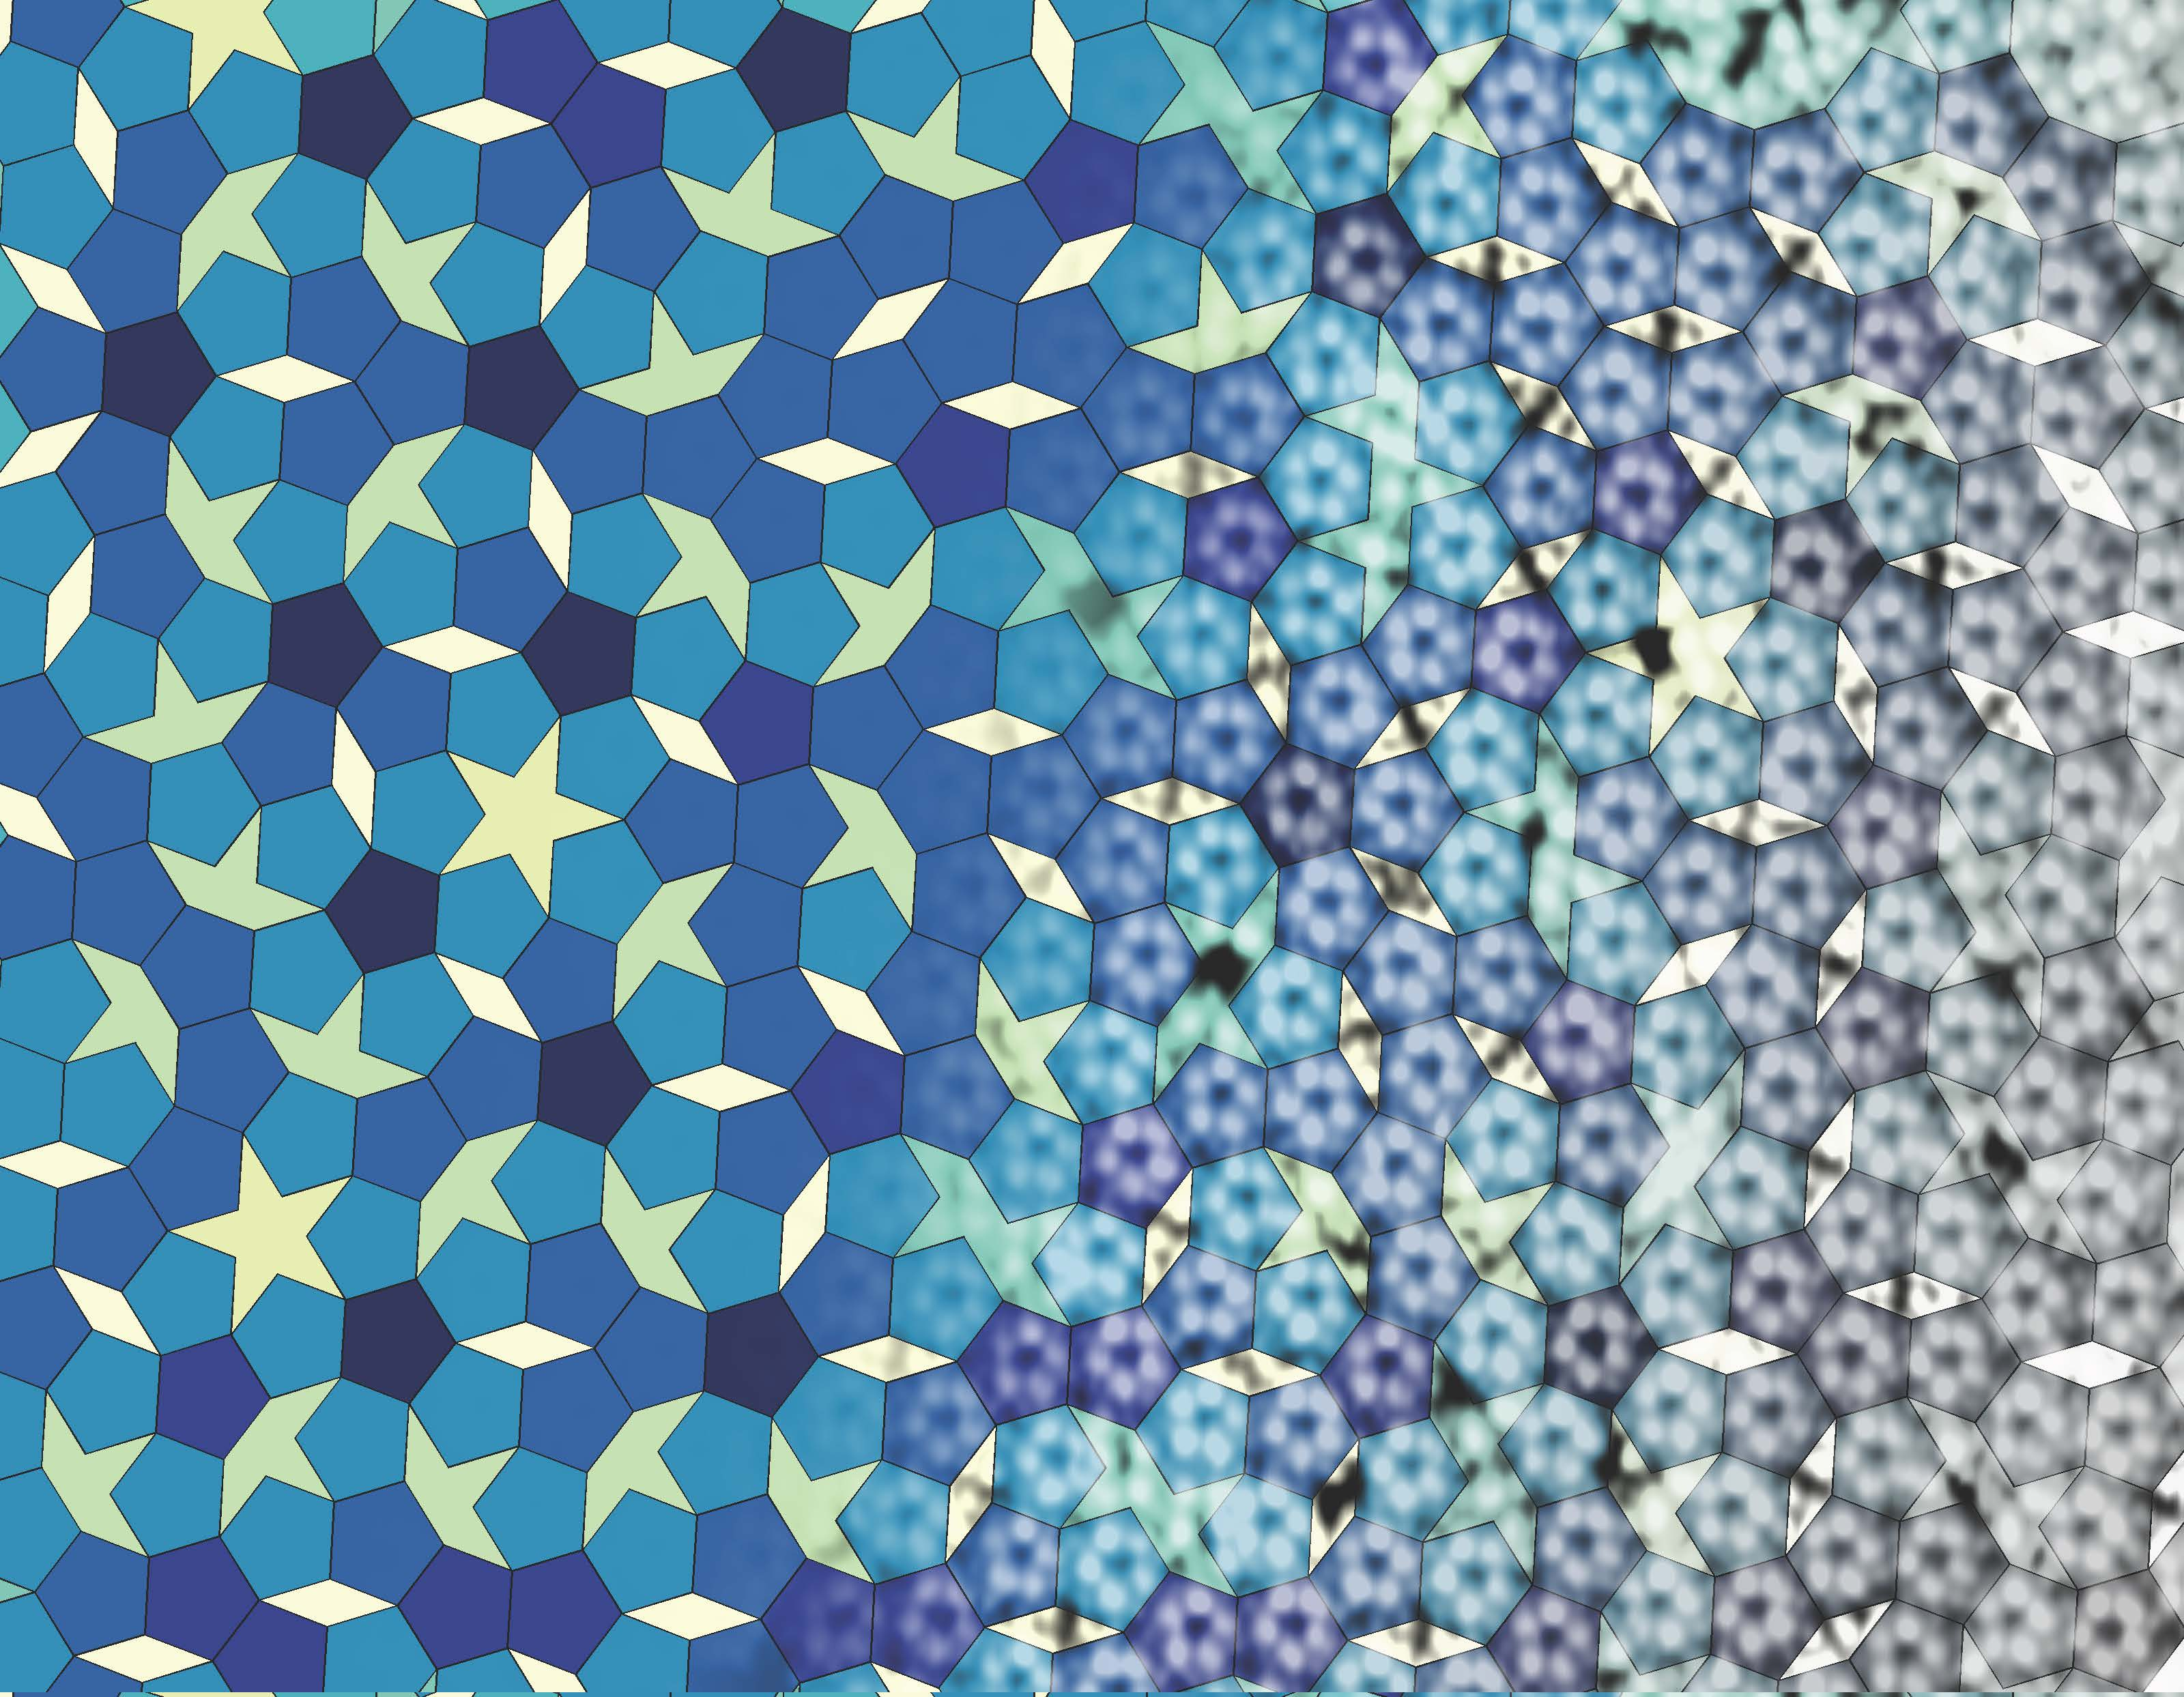
\includegraphics[scale=0.22]{img/wasio.jpg}
		
		\ss{Un quasicristal 2D de molécules} \ss{(voir \url{doi:10.1038/nature12993})}
	\>
\)

\begin{itemize}
	\item De nombreux alliages métalliques sont quasipériodiques sous de bonnes conditions
	\item Seul un exemple connu dans la nature: la météorite de Khatyrka  (voir \url{doi:10.1126/science.1170827 }). 
\end{itemize}
\end{frame}

\begin{frame}{Conduction électrique d'une chaîne d'atomes}


\(
	\<{6cm}
		\centering
		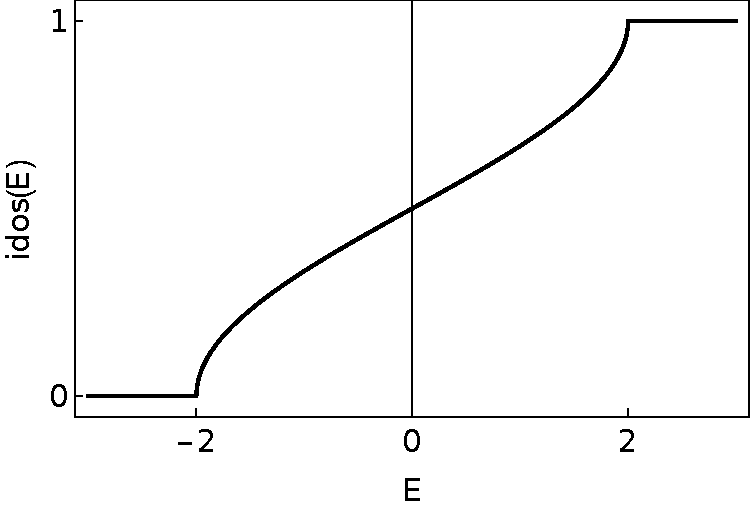
\includegraphics[scale=0.4]{img/idos_chaine_periodique.pdf}
		
		\ss{Densité d'états intégrée de la chaîne périodique}
		\ss{(Amplitude de saut $t=1$)}
	\>
	\<{6cm}
		\centering
		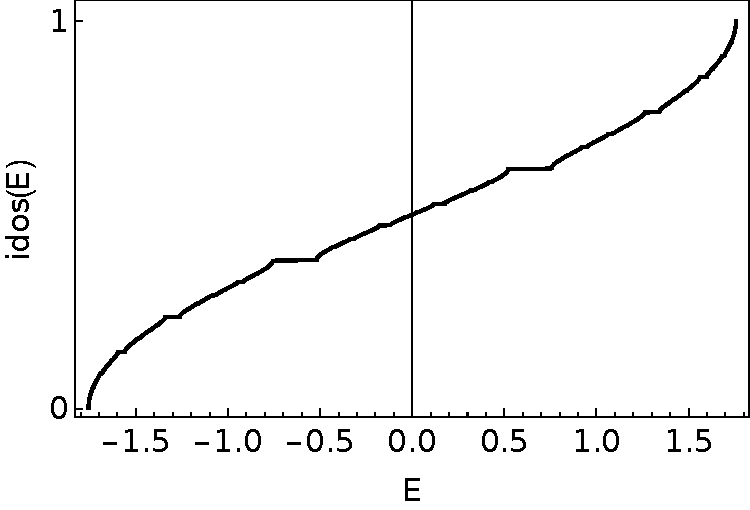
\includegraphics[scale=0.4]{img/idos_fibo.pdf}
		
		\ss{Densité d'états intégrée de la chaîne de Fibonacci} 
		\ss{(Amplitudes de saut $t_B = 1$, $t_A = 0.8$)}
		%\ss{(see \url{doi:10.1007/BF01127714})}
	\>
\)

\(
	\<{6cm}
		\centering
		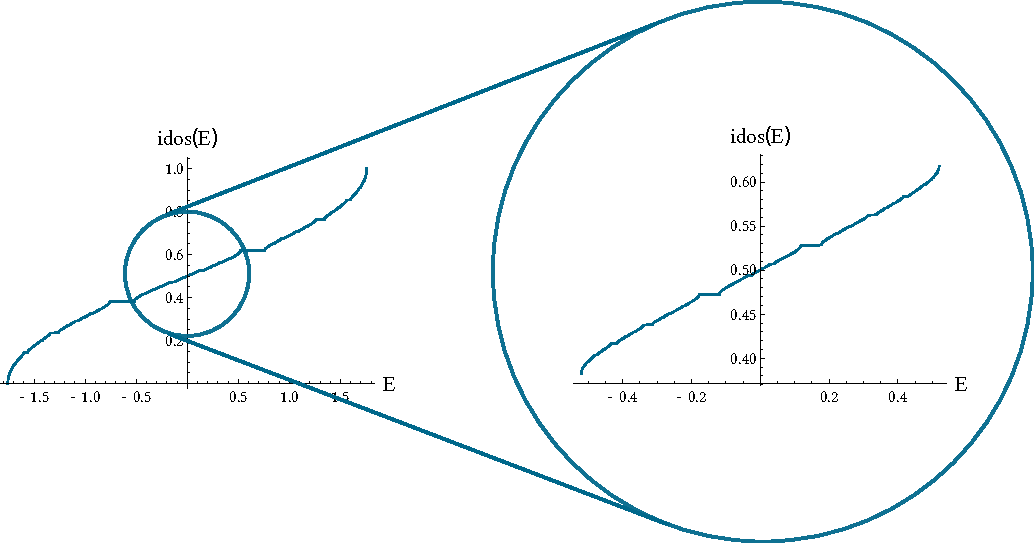
\includegraphics[scale=0.35]{img/idos.pdf}
	\>
	\<{6cm}
\begin{itemize}
	\item Le courant passe si $E_\text{incident} \notin \text{plateau de l'idos}$.
	\item Chaîne périodique : courant si $E_\text{incident} \in [-2t, 2t]$.
	\item Chaîne quasi : courant si $E_\text{incident} \in \text{ensemble de Cantor}$ (voir \emph{Niu \& Nori, PRB 1990})
\end{itemize}
	\>
\)

\end{frame}

\begin{frame}{État central d'une chaîne}

{\centering
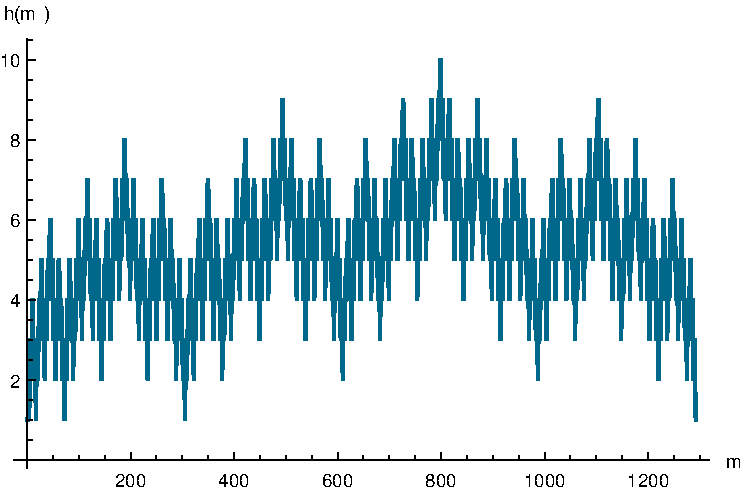
\includegraphics[scale=.7]{img/heights.pdf}

\ss{La fonction de hauteur sur un morceau de la chaîne de Fibonacci}

}

\begin{itemize}
	\item La fonction flèche est quasipériodique.
	\item Son intégrale, la fonction de hauteur, croît en $\sqrt{\log L}$.
\end{itemize}
\end{frame}

\begin{frame}{État central}

{\centering
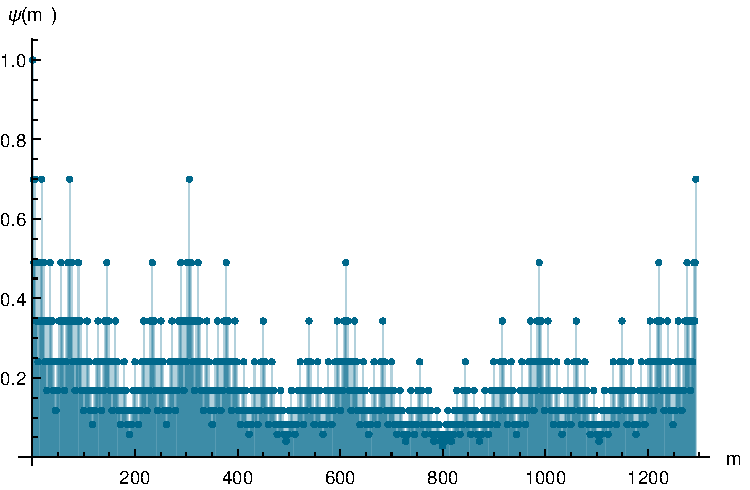
\includegraphics[scale=.8]{img/wavefunction.pdf}

}

\end{frame}

\begin{frame}{Recap}

\begin{itemize}
	\item Wavefunction construction involves a geometrical quasiperiodic function,
	\item Its integral, the height function, has logarithmic growth,
	\item This implies power law behavior of the wavefunction,
	\item The wavefunction is somewhat inbetween localized and extended.
\end{itemize}
$\rightarrow$ We will find again all theses features in the Ammann-Beenker case.
\end{frame}

\end{document}